\documentclass[12pt,letterpaper]{beamer}
\usetheme{Copenhagen}
\usecolortheme{seahorse}
\setbeamertemplate{section in toc}{\inserttocsection}

\usepackage[utf8]{inputenc}
\usepackage{amsmath}
\usepackage{amsfonts}
\usepackage{amssymb}
\usepackage{graphicx}
\graphicspath{ {./images/} }
\usepackage{hyperref}
\hypersetup{
    colorlinks=true,
    linkcolor=blue,
    filecolor=magenta,      
    urlcolor=cyan,
    pdftitle={Overleaf Example},
    pdfpagemode=FullScreen,
}
\title[Robotics I]
{ENGR 3421: ROBOTICS I}
\subtitle{Into the Autonomous Ground Vehicle}

\author[Zhang, Lin]
{Dr. Lin Zhang}
\institute[UCA] % (optional)
{
  Department of Physics and Astronomy\\
  University of Central Arkansas
}
\date[Robotics1 2021] % (optional)
{August 24, 2021}
\logo{
\includegraphics[height=1cm]{uca_bear_logo.png}}


%End of title page configuration block
%------------------------------------------------------------

%------------------------------------------------------------
%The next block of commands puts the table of contents at the beginning of each section and highlights the current section:

\AtBeginSection[]
{
  \begin{frame}
    \frametitle{Outline}
    \tableofcontents[currentsection]
  \end{frame}
}
%------------------------------------------------------------

\begin{document}

%The next statement creates the title page.
\frame{\titlepage}

%---------------------------------------------------------
%This block of code is for the table of contents after the title page
\begin{frame}
\frametitle{Outline}
\tableofcontents
\end{frame}
%---------------------------------------------------------


\section{Review}

\begin{frame}{Safety}
    \begin{alertblock}{Safe First!}
        Don't forget eyes and hands protection!
    \end{alertblock}
    We have gloves and first aid kit now.
\end{frame}

\begin{frame}{Version Control}
    \begin{itemize}
        \item Github provides hosting service.
        \item \href{https://git-scm.com/about}{Git} controls versions.   
    \end{itemize}        
    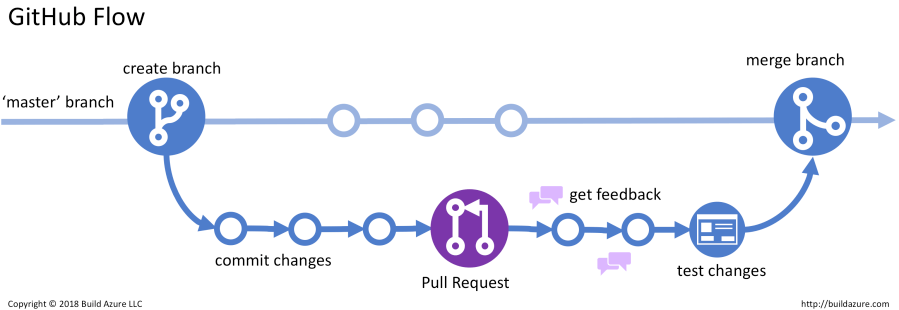
\includegraphics[width=.65\textwidth]{git_flow}
    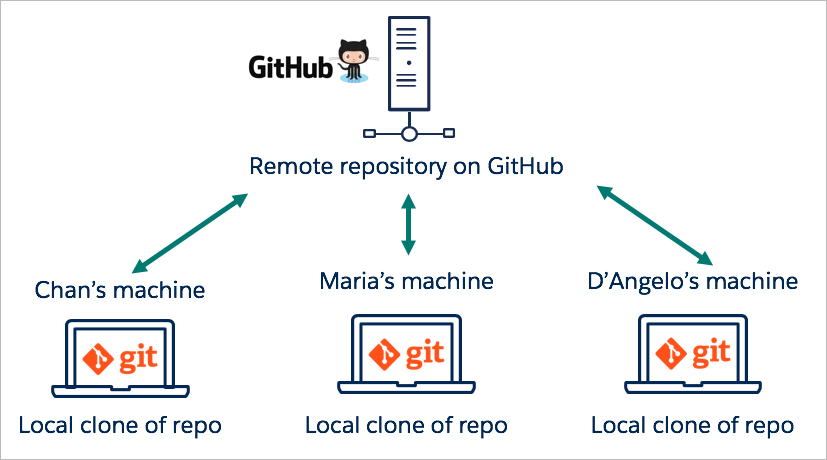
\includegraphics[width=.3\textwidth]{github_and_clones}
\end{frame}

\begin{frame}{Version Control}
    \begin{itemize}
        \item Getting started \href{https://docs.github.com/en/get-started}{guides} and \href{https://guides.github.com/activities/hello-world/}{Hello World}. 
        \item Alternatives: 
        \begin{itemize}
            \item \href{https://about.gitlab.com/}{GitLab}
            \item \href{https://bitbucket.org/product}{Bitbucket}
        \end{itemize}
    \end{itemize}
\end{frame}

\begin{frame}{DC Motor}

\begin{columns}

\column{0.5\textwidth}
% Figure here
\begin{figure}
    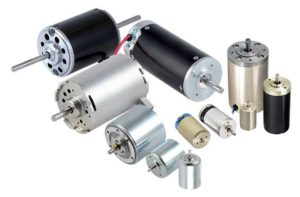
\includegraphics[width=.5\textwidth]{dc_motors}
\end{figure}

\column{0.5\textwidth}
{\small A DC motor is any of a class of rotary electrical motors that converts direct current electrical energy into mechanical energy.} 
{\scriptsize 
\begin{itemize}
    \item Simple.
    \item Low cost.
    \item High efficiency.
    \item No direction.
    \item Pair with reducer to achieve different behavior.
    \item Many applications: toys, ceiling fans, hydraulic pumps, electric cars/bikes, robots ...
\end{itemize}
}

\end{columns}
\hfill \\
A great explanation of \href{https://youtu.be/CWulQ1ZSE3c}{how does a DC motor works}.

\end{frame}

\begin{frame}
    \centering Let's have a race!
\end{frame}

\section{Raspberry Pi}
\begin{frame}{Introduction to Raspberry Pi}
    The Raspberry Pi is a low cost, credit-card sized computer. It’s capable of doing everything you’d expect a desktop computer to do. \\
    Raspberry Pi  has the ability to interact with the outside world, and has been used in a wide array of digital maker projects, from music machines and parent detectors to weather stations and tweeting birdhouses with infra-red cameras. 
\end{frame}

%---------------------------------------------------------
% \begin{frame}{In Scientific/Engineering Research}
    % A robot is a machine—especially one programmable by a computer—capable of carrying out a complex series of actions automatically. 
    % 
    % \href{https://youtu.be/tF4DML7FIWk}{Humanoid} \\
    % \href{https://youtu.be/9j2a1oAHDL8}{Quadrupedal robot} \\
    % \href{https://youtu.be/-q8D7BcLjac}{Spherical robot} \\
    % \href{https://youtu.be/hUE8o056Cpc}{Flapping robot} \\
    % \href{https://youtu.be/Hebpmadjqn8}{Quadrotor $/$ Drone} \\
    % \href{https://youtu.be/4WOOwesIkss}{Underwater robot} \\
    % \href{https://youtu.be/qevIIQHrJZg}{Soft robot} \\
    % \href{https://youtu.be/5qqsMjy8Rx0}{Extra-terrestrial rover} \\
    % \href{https://youtu.be/m-LP4qpOLl0}{You name it...}
% 
% \end{frame}
% 
% \begin{frame}{Autonomous Ground Vehicle (AGV)}
    % A.k.a. automated guided vehicle, mobile robot, unmanned ground vehicle (UGV). 
% 
    % \href{https://youtu.be/fmVWLr0X1Sk}{Self-driving cars} \\ 
    % \href{https://youtu.be/dagjQW_jgtE}{Delivery robots} \\
    % \href{https://youtu.be/IMPbKVb8y8s}{Warehouse robots} 
% 
% \end{frame}
% 
% \begin{frame}{}
    % \href{https://youtu.be/EezdinoG4mk}{Build it, Break it, Fix it}
    % 
% \end{frame}
% 
% %----
% \section{Our Robot}
% 
% \begin{frame}
% \frametitle{Our Robot}
% 
% \begin{columns}
% 
% \column{0.5\textwidth}
% % Figure here
% \begin{figure}
    % 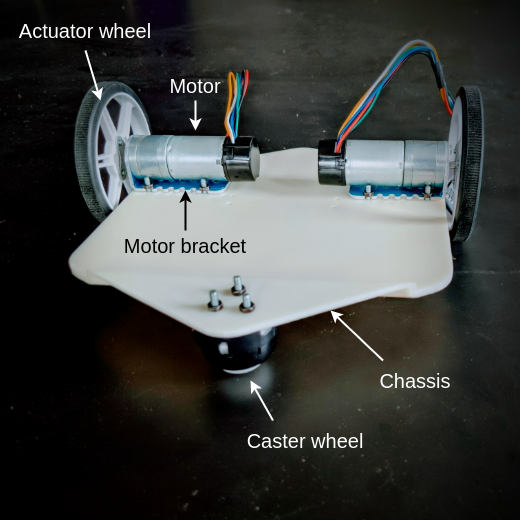
\includegraphics[width=0.8\textwidth]{3421bot}
% \end{figure}
% 
% \column{0.5\textwidth}
% Most parts (all except the chassis) are purchased from \href{https://www.pololu.com/}{Pololu}
% {\scriptsize 
% \begin{itemize}
    % \item Chassis (\href{https://github.com/linzhangUCA/robotics1-2021/blob/main/0819/chassis_v3.stl}{3D model})
    % \item \href{https://www.pololu.com/product/2691}{Caster wheel} (Pololu \#: 2691) 
    % \item \href{https://www.pololu.com/product/2676}{Motor brackets} (Pololu \#: 2676)
    % \item \href{https://www.pololu.com/product/4805}{Motor} (Pololu \#: 4805)
    % \item \href{https://www.pololu.com/product/3690}{Actuator wheel} (Pololu \#: 3690)
% \end{itemize}
% 
% }
% \begin{block}
% \footnotesize 3D printer @ CCCS 112
% \end{block}
% 
% \end{columns}
% 
% \end{frame}
% %---------------------------------------------------------
% 
% 
% 
% \section{Github Classroom}
% \begin{frame}{Github}
    % \href{https://github.com}{GitHub} is a website and cloud-based service that helps developers store and manage their code, as well as track and control changes to their code. 
% \end{frame}
% 
% \begin{frame}{Github Classroom}
% \begin{itemize}
    % \item \href{https://classroom.github.com}{GitHub Classroom} automates repository creation and access control, making it easy to distribute starter code and collect assignments on GitHub.
    % \item This is the place you'll complete most (if not all) of your assignments.
% \end{itemize}
% 
% 
% \begin{alertblock}{Note}
% {\footnotesize 
% \begin{itemize}
        % \item Access Github Classroom: \href{https://classroom.github.com}{https://classroom.github.com}
        % \item Check your email for my invitation.
    % \end{itemize}
% }
% \end{alertblock}   
% 
% \end{frame}
% 
\end{document}
